\documentclass[a4paper,10pt]{article}
%-----------------------------------------------------------
\usepackage[top=0.75in, bottom=0.75in, left=0.55in, right=0.85in]{geometry}
\usepackage{graphicx}
\usepackage{url}
\usepackage{palatino}
\usepackage{tabularx}
\fontfamily{Calibri}
\selectfont

\usepackage[T1]{fontenc}
\usepackage
%[ansinew]
[utf8]
{inputenc}

\usepackage{color}
\definecolor{mygrey}{gray}{0.75}
\textheight=9.75in
\raggedbottom

\setlength{\tabcolsep}{0in}
\newcommand{\isep}{-2 pt}
\newcommand{\lsep}{-0.5cm}
\newcommand{\psep}{-0.6cm}
\renewcommand{\labelitemii}{$\circ$}

\pagestyle{empty}
%------------------------------------------------------------
%Custom commands
\newcommand{\resitem}[1]{\item #1 \vspace{-2pt}}
\newcommand{\resheading}[1]{{\small \colorbox{mygrey}{\begin{minipage}{0.975\textwidth}{\textbf{#1 \vphantom{p\^{E}}}}\end{minipage}}}}
\newcommand{\ressubheading}[3]{
\begin{tabular*}{6.62in}{l @{\extracolsep{\fill}} r}
	\textsc{{\textbf{#1}}} & \textsc{\textit{[#2]}} \\
\end{tabular*}\vspace{-8pt}}
%-----------------------------------------------------------

\begin{document}
\hspace{0.5cm}\\[-0.2cm]
\begin{flushright}
\large
\textbf{Mukesh P} \\
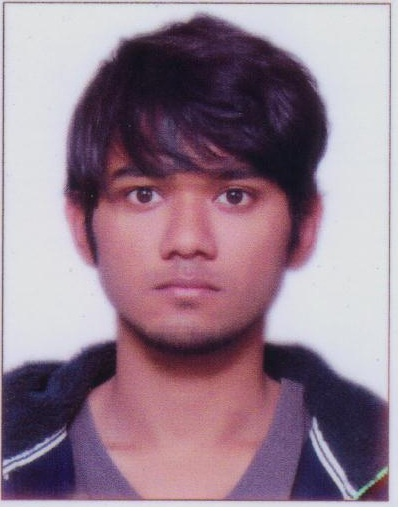
\includegraphics[width = 30mm]{a.jpg}
\end{flushright}

\indent \resheading{\textbf{CONTACT INFORMATION} }\\[\lsep]
\\ \\

\indent\begin{tabular}{@{}p{3.5in}p{3.5in}}
Plot no. 12, Road no. 14, &{Phone No.:} +91-9869365330 \\ 
Sector 12, New Panvel,	&  {Email-id:}mukesh85tek@gmail.com \\
Navi Mumbai, Maharashtra - 410206   \\
\end{tabular}

\indent\resheading{\textbf{CAREER OBJECTIVE} }\\[\lsep]
\\ \\
\indent To be a part of an organization that provides an atmosphere of mutual growth and benefits, where I can \indent show  my talent and potential.


\indent\resheading{\textbf{EDUCATION} }\\[\lsep]
\\ \\
\indent \begin{tabular}{ l @{\hskip 0.15in} l @{\hskip 0.15in} l @{\hskip 0.15in} l @{\hskip 0.15in} l}
	\hline
	\textbf{Examination} & \textbf{University} & \textbf{Institute} & \textbf{Year} & \textbf{CPI} \\
	\hline
	10th Board & CBSE & D.A.V. Public School & 2010 & 9.8 \\
	\hline
	12th Board & CBSE & Shiv Jyoti School & 2012 & 81\% \\
	\hline
	B.E. & Mumbai University & Fr. Rodrigues Institute of technology, Vashi & 2016 & 7.7\\
	\hline
\end{tabular}
\\ \\

\resheading{\textbf{PROJECTS} }\\[\lsep]
\\ \\
\begin{enumerate}
		\item COLLEGE INTRANET
		\subitem Objective: To make sharing of data easier between students and teachers. \\
		\indent \indent Languages and tools: Android, Java Swing.
		
		\item NETWORK PERFORMANCE MONITOR
		\subitem Objective: To calculate the throughput of a system when different types of connection are established.
		\indent \indent Languages and tools: Java Swing.
\end{enumerate}

\resheading{\textbf{TRAINING AND INTERNSHIP} }\\[\lsep]
\\ \\
\begin{itemize}
					\item ETHICAL HACKING: Attended a 15 day workshop on ethical hacking held in IIT Bombay.
					\item OpenGL:
					Attended a 3 day workshop at college held under Cryptex.
					\item No internships yet
\end{itemize}

\resheading{\textbf{RESEARCH PUBLICATIONS} }\\[\lsep]
\\ \\
\begin{enumerate}
		\item No research publications yet. \\ \\ \\
\end{enumerate}

\resheading{\textbf{TECHNICAL SKILLS} }\\[\lsep]
\\ \\
\begin{itemize}
	\item \noindent \textbf{Languages} (C, C++, Java, Python, AS3)
	\item \noindent \textbf{Database} (MySQL)
	\item \noindent \textbf{Script} (HTML, CSS, PHP) 
	\item \noindent \textbf{Tools} (Eclipse, Android Studio, lex, yacc \LaTeX, Packet Tracer, NSG, Adobe CSS).
	
\end{itemize}

\resheading{\textbf{SOFT SKILLS} }\\[\lsep]
\\ \\
\begin{enumerate}
		\item \noindent Skilled in delegating tasks among team members and motivating them.
		\item \noindent Efficient in developing a schedule.
		\item \noindent Capable of adapting to different environments.
		\item \noindent Proficient in solving problems.
		\item \noindent Good at communicating with people belonging to different communities.
		\item \noindent Ability to work independently.
\end{enumerate}

\resheading{\textbf{EXTRA CURRICULAR} }\\[\lsep]
\\ \\


\begin{itemize}
		\item \noindent In college festival...
		\begin{itemize}
			\item Stood first in food fest.
			\item Won swimming relays.
			\item Stood second in solo-instrumentals.
			\item Won LAN gaming competition.
		\end{itemize}
\end{itemize}

\resheading{\textbf{CO-CURRICULAR} }\\[\lsep]
\\ \\
\begin{enumerate}
			\item \noindent Chosen for second round of Code-vita twice.
			\item \noindent Chosen amongst the top 14 students in "CSI Discover Thinking 3rd National Programming Contest 2015" held by Computer society of India.
			\item \noindent lead the team to victory in e-Yantra Robotics Competition(eYRC)-2014.
			\item \noindent Conducted a workshop on Android development under Cryptex-2015.
\end{enumerate}

\resheading{\textbf{PERSONAL INFORMATION} }\\[\lsep]
\\ \\
\indent Father’s Name: Prakash J. \\
\indent Mother’s Name: Hema P. \\
\indent Sex: Male \\
\indent Date of Birth:6th February 1995 \\
\indent Nationality: Indian \\
\indent Marital Status: Single \\

\resheading{\textbf{REFERENCE} }\\[\lsep]
\\ \\


\resheading{\textbf{DECLARATION} }\\[\lsep]
\\ \\


\resheading{\textbf{DATE} }\\[\lsep]
\\ \\

\end{document}

